\documentclass[
    a4paper,
    twocolumn,
]{article}

% Table insertions
% --------------------------------------------------
\usepackage{graphics}

% Image insertions
% --------------------------------------------------
\usepackage{graphicx}
\usepackage[belowskip=-3pt,aboveskip=8pt]{caption}
\graphicspath{{./images/}}

% Input and font encoding
% --------------------------------------------------
\usepackage[utf8]{inputenc}
\usepackage[T1]{fontenc}

% biblatex --- Bibliography setup
% --------------------------------------------------
\usepackage[
    backend=biber,
    style=numeric,
    sorting=none,
]{biblatex}

\addbibresource{sources.bib}

% hyperref --- Hyperlinks in PDF
% --------------------------------------------------
\usepackage[pdfusetitle]{hyperref}

% Set colors of links
\hypersetup{
    colorlinks=true,
    linkcolor=magenta,
    citecolor=,
    urlcolor=blue,
}

% Allow line-breaks in links and URLs
\hypersetup{breaklinks=true}

% Use the normal document font for URLs rather than monospace
\urlstyle{same}

% Document Metadata
% --------------------------------------------------
\title{INF3200: Mandatory Assignment 2}
\author{Yasiru Rathsara Witharanage}
\date{\today}

% Document
% --------------------------------------------------
\begin{document}

\maketitle

\begin{abstract}
    \textbf{In the context of distributed systems, the term stability is trivial as the existence of individual nodes are not predefined and fixed. Hence it is significantly important to address the issue of inconsistent structure dynamically while minimizing the adverse impact on performance of the system thus providing transparency to the end-user. This paper discusses a solution to this complication of ever-changing participants of a key-value store based on chord~\cite{1} along with the experiments conducted to measure its performance and behavior.}
\end{abstract}

\section{Introduction}

In this study, a distributed hash table was implemented based on chord which uses a ring topology where each node in the system is only aware of its predecessor and successor initially. A node is responsible for storing and retrieving of any key-value pair that belongs to its bucket space based on node id. These keys and node ids are first hashed using SHA256~\cite{2} algorithm in order to minimize the collision of two separate nodes and to utilize the potential of supporting an enormously large distributed store.\\

Main objective of this study is to build a chord network resilient to dynamic changes which can be occurred due to joining and leaving of nodes. This adaptation also includes coping against crashing of nodes without any prior notification and re-construct network leaving these out-of-reach nodes. Moreover, it should be able to detect these left out nodes and include them in the network whenever they are reachable again.\\

Following HTTP endpoints are exposed to serve store functionalities as well as to cope with dynamically changing structure of server nodes. Note that nodes are not aware of cluster information and cluster-info endpoint circulates an HTTP request around the ring structure to collect necessary data. 

\begin{itemize}
	\item PUT /storage/key - stores a value provided in the raw body
	\item GET /storage/key - returns the value of a key (returned in raw body)
	\item POST /join?nprime=HOST:PORT - joins the network using an existing node
	\item POST /leave - leaves out the requested node from network
	\item GET /neighbors - returns the neighbours of a node
	\item GET /node-info - returns a JSON response of requested node information
	\item GET /cluster-info - returns cluster information
\end{itemize}

\section{Project Description}
\subsection{Design}

Each individual node in the network is given an id based on the SHA256 hash value of its own hostname and is only aware of its neighbours, i.e. predecessor and successor. These values can be configured before the execution of a node. \\

Whenever a query is received by a node, it initially checks whether the requested key belongs to itself and if not, it proceeds to the immediate successor. This process is iterated until the correct node for key is discovered and the corresponding response is returned along the same route. \\

When joining the network, a request is sent to the new node along with an existing node in the cluster and thus a join is initiated to this entry point where it starts circulating the request until the corresponding successor of new node is reached. This successor then updates its new predecessor while notifying the ex-predecessor to update its successor. Once this circulation is successful, neighbors of the new node will be returned by the response and updated in the joining node.\\

On the other hand, a node notifies both its predecessor and successor upon leaving, to update their neighbors accordingly. Since these two requests are independent of each other, they can be executed in parallel thus saving an overhead latency of multiple requests. In both these scenarios, bucket space will be adjusted with respect to the network change. \\

Moreover, a probing mechanism is implemented in each node to detect any out of reach condition of its predecessor and automatically rectify with active nodes by eliminating the crashed node. Once a crash is recognized, the successor will circulate an internal HTTP request until the last active node is found and thus updating a new connection between these two nodes. Immediate successors also keep track of these disconnected nodes to add once they become reachable again and this check is done in the order of proximity, i.e. closest lost node will be checked before the rest and so on. However, this system does not support the migration of existing key-value pairs when changing the components of network.

\subsection{Implementation}

Golang was used for the implementation of chord with a flat-hierarchical code structure and different layers for each functionality. HTTP endpoints listed previously were implemented in HTTP layer while node layer contains details (node id, predecessor, successor) related with the node along with validating key function. SHA256 was used for hashing of both key and node id to match with relevant buckets. A separate HTTP client was used in neighbour layer to proceed any request with a key that does not belong to the corresponding node. All key-value entry pairs are stored in an in-memory map which is specifically designed for concurrent use.\\

A sample set is given below for the configuration values of parameters required by the implementation but however user is allowed to provide his own desired values for service configurations. 

\begin{verbatim}
# service configs
port: 52520
request_timeout_sec: 5
ttl_min: 180

# neighbor configs
probe_interval_sec: 10
detect_crash_timeout_sec: 2

# logger configs
colors_enabled: true
log_level: "TRACE"
file_path: true
\end{verbatim}

\texttt{request\_timeout\_sec} refers to the waiting time of a single HTTP request by a node in seconds and each node has a TTL in minutes for the self-termination configured by \texttt{ttl\_min}. \texttt{probe\_interval\_sec} is used as the time interval in which each node is checking if their immediate predecessors are reachable. A separate HTTP client is used to detect whether a successor is not responsive in finding the last active node triggered by a node crash. This detection is done with a timeout configured by \texttt{detect\_crash\_timeout\_sec}.

\section{Evaluation}

Several experiments were carried out to evaluate performance and stability of network with dynamic changes in the structure. First experiment was conducted to measure the time consumption of network to stabilize after varying number of joins of nodes. This was achieved by sending sequential join requests to every node and logging timestamps with each node's action. Total time to stabilize was taken as the time difference between initial join action and the last neighbor update by a node. Finally cluster information response was considered to ensure that the network consisted of the desired number of nodes.\\


Table 1 and 2 provide details about hardware specifications of nodes and sets of nodes used in each experiment.

\begin{table}[!ht]
\renewcommand{\arraystretch}{1.4}
\centering
\resizebox{\columnwidth}{!}{%
\begin{tabular}{|c | c | c | c | c | c|} 
	\hline
	Node ID & Hostname & Model & CPUs & Cores & Processors\\
	\hline
	0 & compute-6-18 & Lenovo P310 & 1 & 4 & 4 \\ 
	\hline
	1 & compute-8-6 & Lenovo m93p & 1 & 4 & 8 \\ 
	\hline
	2 & compute-3-28 & Dell T3600 & 1 & 4 & 4 \\ 
	\hline
	3 & compute-6-21 & Lenovo P310 & 1 & 4 & 4 \\ 
	\hline
	4 & compute-3-23 & Dell T3600 & 1 & 4 & 4 \\ 
	\hline
	5 & compute-8-7 & Lenovo m93p & 1 & 4 & 8 \\ 
	\hline
	6 & compute-6-34 & Lenovo P310 & 1 & 4 & 4 \\ 
	\hline
	7 & compute-6-16 & Lenovo P310 & 1 & 4 & 4 \\ 
	\hline
	8 & compute-6-17 & Lenovo P310 & 1 & 4 & 4 \\ 
	\hline
	9 & compute-3-21 & Dell T3600 & 1 & 4 & 4 \\ 
	\hline
	10 & compute-8-5 & Lenovo m93p & 1 & 4 & 8 \\ 
	\hline
	11 & compute-6-22 & Lenovo P310 & 1 & 4 & 4 \\ 
	\hline
	12 & compute-6-15 & Lenovo P310 & 1 & 4 & 4 \\ 
	\hline
	13 & compute-8-8 & Lenovo m93p & 1 & 4 & 8 \\ 
	\hline
	14 & compute-6-19 & Lenovo P310 & 1 & 4 & 4 \\ 
	\hline
	15 & compute-3-0 & Dell T3600 & 1 & 4 & 4 \\ 
	\hline
\end{tabular}%
}
\caption{Hardware specification of nodes}
\end{table}

\begin{table}[!ht]
	\renewcommand{\arraystretch}{1.1}
	\centering
	\resizebox{\columnwidth}{!}{%
		\begin{tabular}{|c | l|} 
			\hline
			Number of nodes &\multicolumn{1}{|c|}{Node IDs} \\
			\hline
			1 & 10 \\ 
			\hline
			2 & 0, 7 \\
			\hline
			4 & 2, 5, 8, 11 \\
			\hline
			8 & 0, 1, 4, 6, 8, 9, 10, 13 \\
			\hline
			16 & 0, 1, 2, 3, 4, 5, 6, 7, 8, 9, 10, 11, 12, 13, 14, 15 \\
			\hline
		\end{tabular}%
	}
	\caption{Nodes used in each experiment}
\end{table}

\section{Results}

Following are the average stabilization times taken for the first experiment in milliseconds with different number of nodes joining to the cluster. 

Following are the average execution times obtained per each query type (GET and PUT) while varying number of queries in the batch and number of nodes in the cluster (Table 3). Note that throughput experiments in clusters with higher number of nodes were limited due to file descriptor limits. Each attempt was done 3 times and the resultant average total latency value was calculated for the average time.

\begin{table}[!ht]
	%\LARGE
	\renewcommand{\arraystretch}{1.5}
	\centering
	\resizebox{\columnwidth}{!}{%
		\begin{tabular}{|c | c | c | c|} 
			\hline
			No. of nodes & No. of requests & Latency-GET(ms) & Latency-PUT(ms) \\
			\hline
			& 16 & 0.2708 & 0.3542 \\
			\cline{2-4}
			1 & 100 & 0.1066 & 0.1133 \\
			\cline{2-4}
			& 1000 & 0.0580 & 0.0553 \\
			\hline
			& 16 & 0.3750 & 0.3958 \\
			\cline{2-4}
			2 & 100 & 0.1267 & 0.1233 \\
			\cline{2-4}
			& 1000 & 0.0630 & 0.0607 \\
			\hline
			& 16 & 0.5833 & 0.6042 \\
			\cline{2-4}
			4 & 100 & 0.1900 & 0.2033 \\
			\cline{2-4}
			& 500 & 0.1007 & 0.1240 \\
			\hline
			& 16 & 0.9167 & 0.9375 \\
			\cline{2-4}
			8 & 100 & 0.2467 & 0.2767 \\
			\cline{2-4}
			& 500 & 0.1653 & 0.1407 \\
			\hline
			& 16 & 1.5417 & 1.4583 \\
			\cline{2-4}
			16 & 100 & 0.3833 & 0.3733 \\
			\cline{2-4}
			& 500 & 0.1693 & 0.1460\\
			\hline
		\end{tabular}%
	}
	\caption{Results of experiments}
\end{table}

\section{Discussion}

Following histograms (Figure 2 and 3) with error bars for standard deviation~\cite{2} were derived by using the above results where y-axis implies the calculated average time and x-axis denotes the experiments in the form of (number of nodes, number of requests).\\

\setlength{\intextsep}{10pt plus 2pt minus 0pt}
\begin{figure}[!ht]
	\centering
	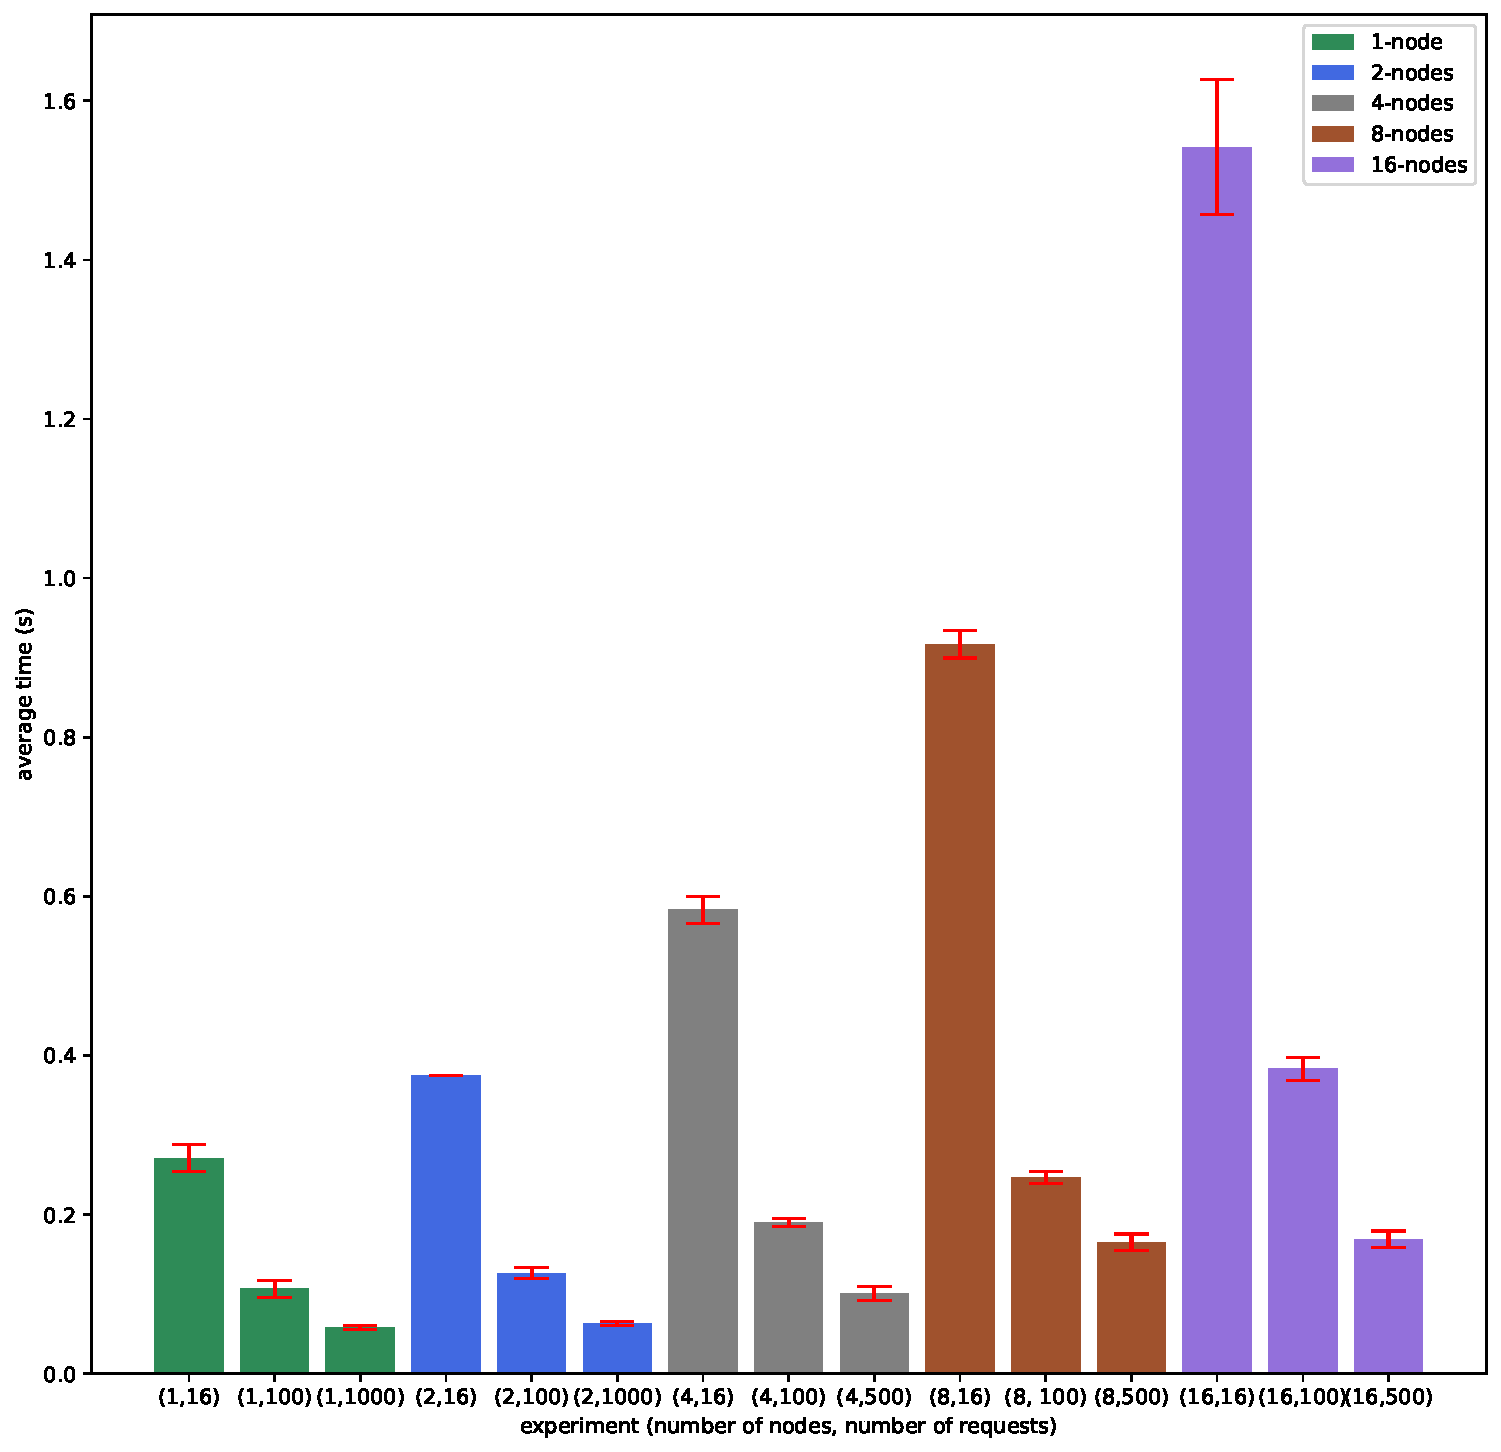
\includegraphics[width=7.5cm, height=5cm]{get.pdf}
	\caption{Histogram of average times for GET requests with different parameters}
\end{figure}

\setlength{\intextsep}{5pt plus 2pt minus 0pt}
\begin{figure}[!ht]
	\centering
	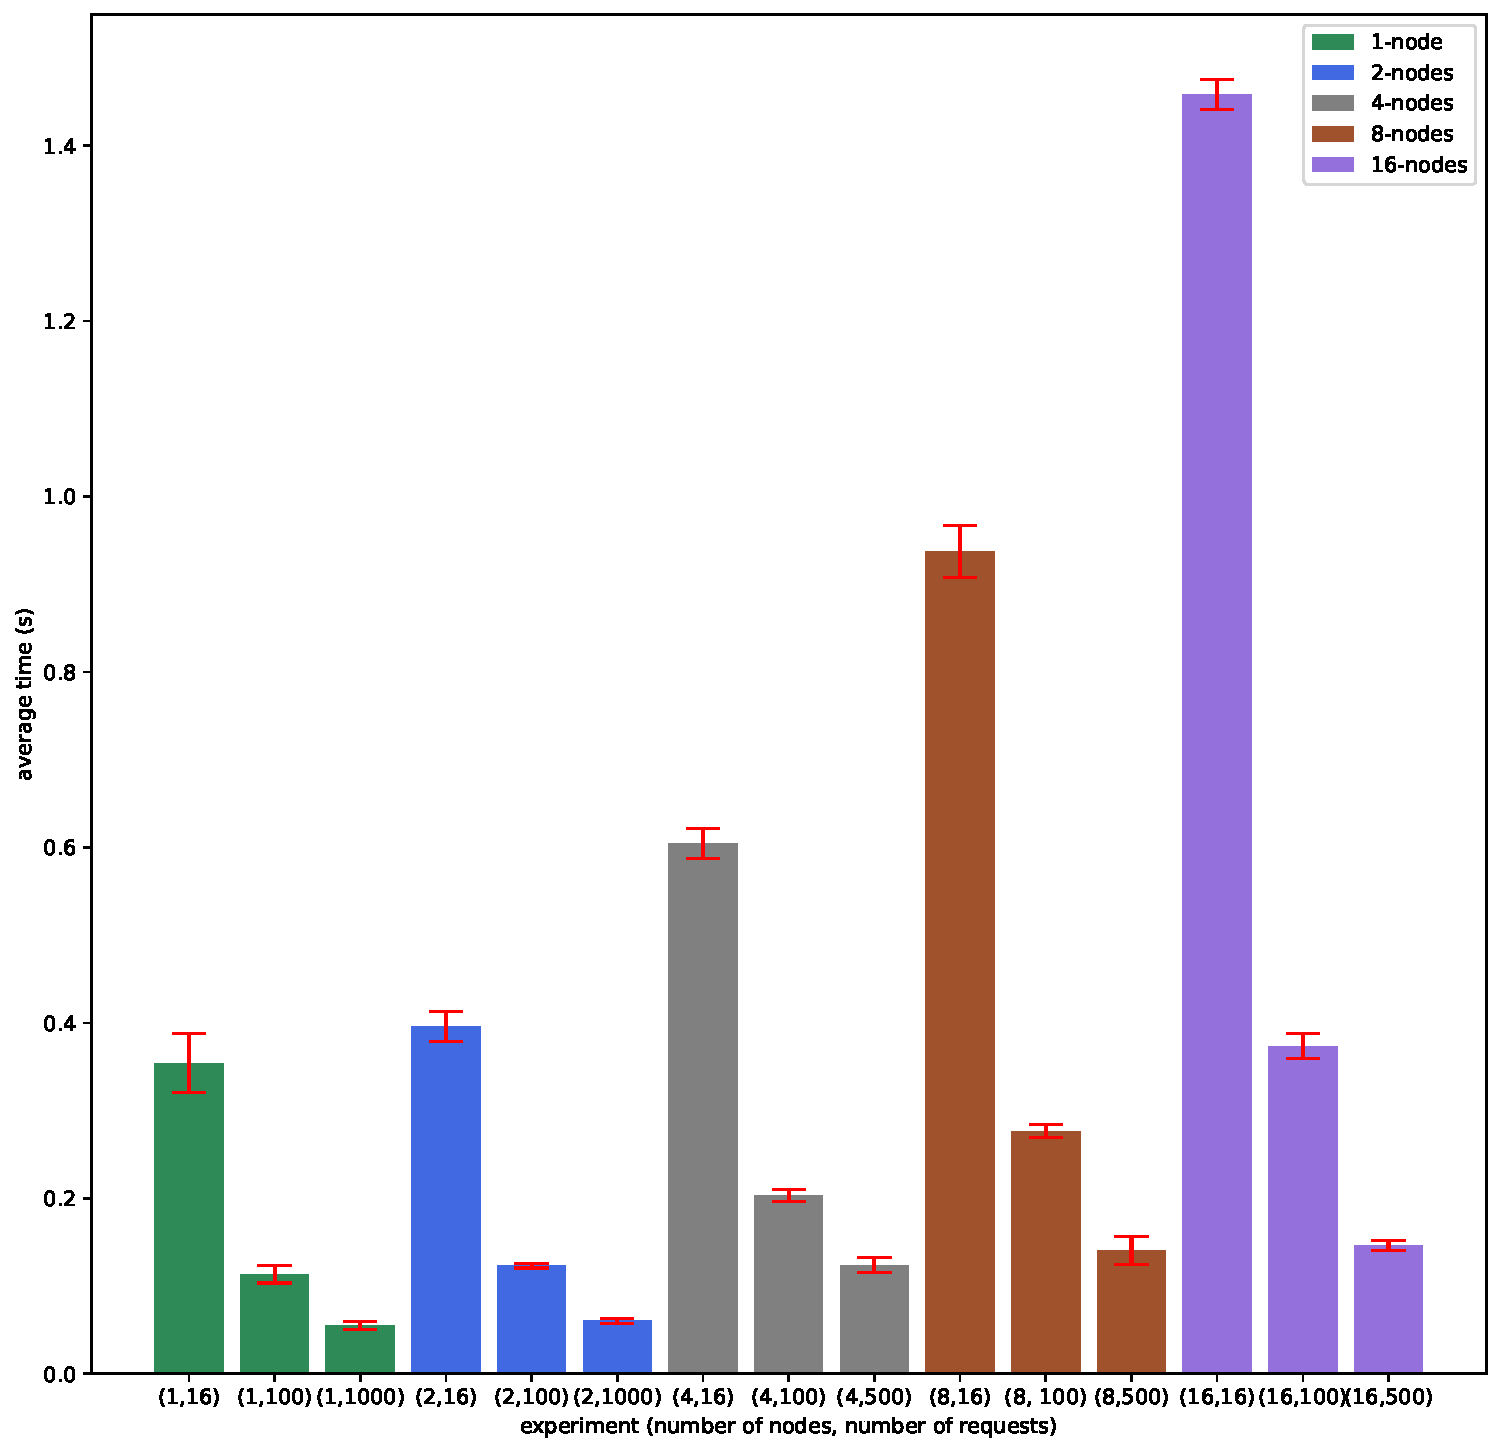
\includegraphics[width=7.5cm, height=5cm]{put.pdf}
	\caption{Histogram of average times for PUT requests with different parameters}
\end{figure}

Line graphs in Figure 4 and 5 were constructed for more precise interpretation and comparison of experiment results.\\

\setlength{\intextsep}{7pt plus 2pt minus 0pt}
\begin{figure}[!ht]
	\centering
	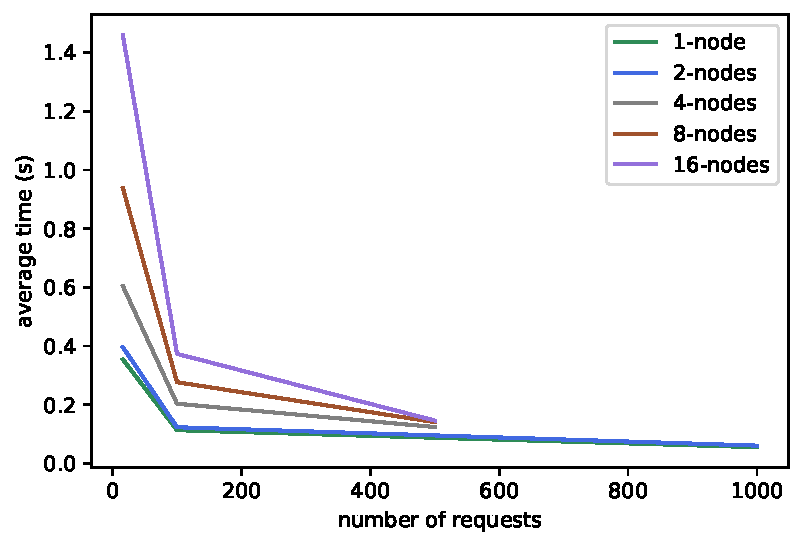
\includegraphics[width=7.5cm, height=5cm]{put_line.pdf}
	\caption{Line graph of average times for PUT requests with different parameters}
\end{figure}

\setlength{\intextsep}{5pt plus 2pt minus 0pt}
\begin{figure}[!ht]
	\centering
	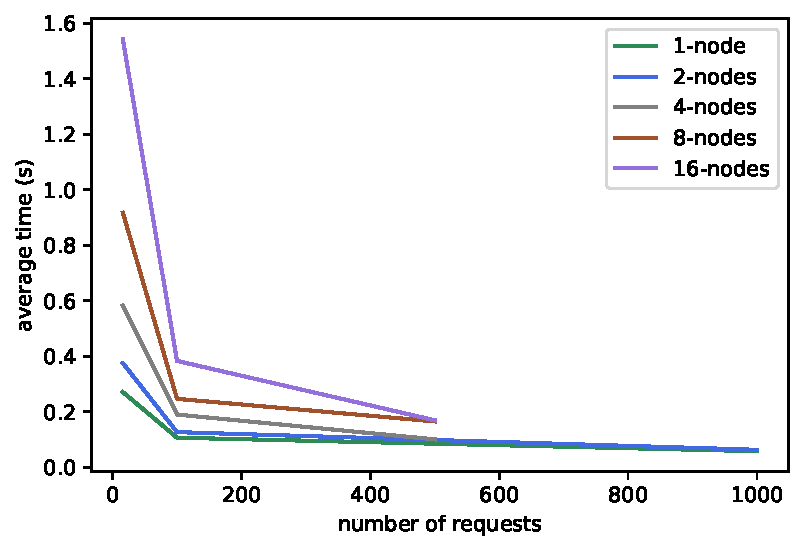
\includegraphics[width=7.5cm, height=5cm]{get_line.pdf}
	\caption{Line graph of average times for GET requests with different parameters}
\end{figure}

By observing these charts, it is obvious that response times increase with number of nodes in the network for a particular batch of requests and can this be explained by the rise in redundant HTTP calls among nodes when a network expands. However, this increasing factor seems to be diminishing when the size of the request batch increases. \\

Furthermore, for a given network with a fixed number of nodes, latency decreases as opposed to number of requests in the batch. A possible reason for this observation could be that the capability of a node to process query requests asynchronously while the rest are still in progress or being circulated in the network and thus maximizing the throughput relatively.\\

This entire behaviour is consistent across both request types (GET and PUT) despite the minor variations in latency. Lower average times are highly possible if the communication among nodes can be replaced with a better approach.

\section{Conclusion}

Finally, it can be concluded that the implemented key-value store is more appropriate when the number of queries is higher in terms of the performance for a given network of nodes. In contrast, number of nodes in the network has a negative impact on the query latency. \\ 

Thus, the distributed key-value store should be designed with a preferable number of nodes such that it addresses the trade-off between performance and other quantitative/non-quantitative measures of a distributed system (scalability, accessibility, load of queries, fault tolerance etc.) depending on the requirements of a given scenario.

\begin{thebibliography}{9}	
	\bibitem{chord}
	Ion Stoica, Robert Morris, David Karger, M. Frans Kaashoek, Hari Balakrishnan (2001) \emph{Chord: A Scalable Peer-to-Peer Lookup Service for Internet Applications }, MIT Laboratory for Computer Science.
	
	\bibitem{error}
	Lee, Dong and In, Junyong and Lee, Sangseok (2015) \emph{Standard deviation and standard error of the mean}, Korean journal of anesthesiology.
\end{thebibliography}

\appendix
\section{Source Code}
\href{https://github.com/YasiruR/dht/tree/master}{Github repository}

\end{document}
